\section{Methods}
\label{sec:methods}

%\subsection{Context and process}

\begin{figure}
\resizebox{\columnwidth}{!}{%
%% For final:
\begin{tikzpicture}
%  \draw[thick] (4,0) node[below={2cm}] {\emph{A.~``mere generation''}}
%                     pic[red, -latex]{darc=100:270:1.3cm:Chicken:Lay:2.4cm:3cm}
%                     pic[red, -latex]{uarc=280:450:1.3cm:Egg:Hatch:1cm:.1cm};
%
  \draw[thick] (4.0,0) node[below={2cm},align=center] {\emph{A.~how to become a writer\footnotemark}}
                      pic[red, -latex]{darc=100:270:1.3cm:{}:{Write for 8 hours a day}:1cm:.3cm}
                      pic[red, -latex]{uarc=280:450:1.3cm:{}:{Read for 8 hours a day}:1cm:.3cm};
%
  \draw[thick](8.5,0) node[below={2cm}] {\emph{B.~``the Other''}}
                     pic[red, -latex]{darc=100:270:1.3cm:Statement:Speak:2.1cm:2.6cm}
                     pic[red, -latex]{uarc=280:450:1.3cm:Response:{Listens and interprets}:.2cm:.1cm};

%  \draw[thick] (4,-5.5) node[below={2.2cm}] {\emph{D.~learning by doing}}
%                        pic[red, -latex]{darc=100:240:1.5cm:Poet:Write:3cm:2.7cm}
%                        pic[red, -latex]{rarc=250:320:1.5cm:Poem:Responds:1cm:.5cm}
%                        pic[red, -latex]{uarc=330:450:1.5cm:Context:Speaks:1cm:.1cm};
%
%
  \draw[thick] (13,0) node[below={2cm}] {\emph{C.~proto-workshop}}
                        pic[red, -latex]{larc=100:180:1.3cm:Poet:Writes:1cm:.2cm}
                        pic[red, -latex]{rarc=190:270:1.3cm:Poem:Responds:1cm:.4cm}
                        pic[red, -latex]{rarc=280:360:1.3cm:Context:Speaks:.7cm:.7cm}
                        pic[red, -latex]{larc=370:450:1.3cm:Reader:Responds:.8cm:.2cm};

%  \draw[thick] (13,-5.5) node[below={2.2cm}] {\emph{F.~how computers work}}
%                       pic[red, -latex]{darc=100:180:1.5cm:{}:Print:1.5cm:1.4cm}
%                       pic[red, -latex]{rarc=190:270:1.5cm:{}:Loop:1cm:1.4cm}
%                       pic[red, -latex]{rarc=280:360:1.5cm:{}:Read:1cm:1.4cm}
%                       pic[red, -latex]{larc=370:450:1.5cm:{}:Eval:1.4cm:.2cm};
% Note:
% controls at end: offset of outer text, followed by offset of inner text
\end{tikzpicture}

%% For quick compiling
% 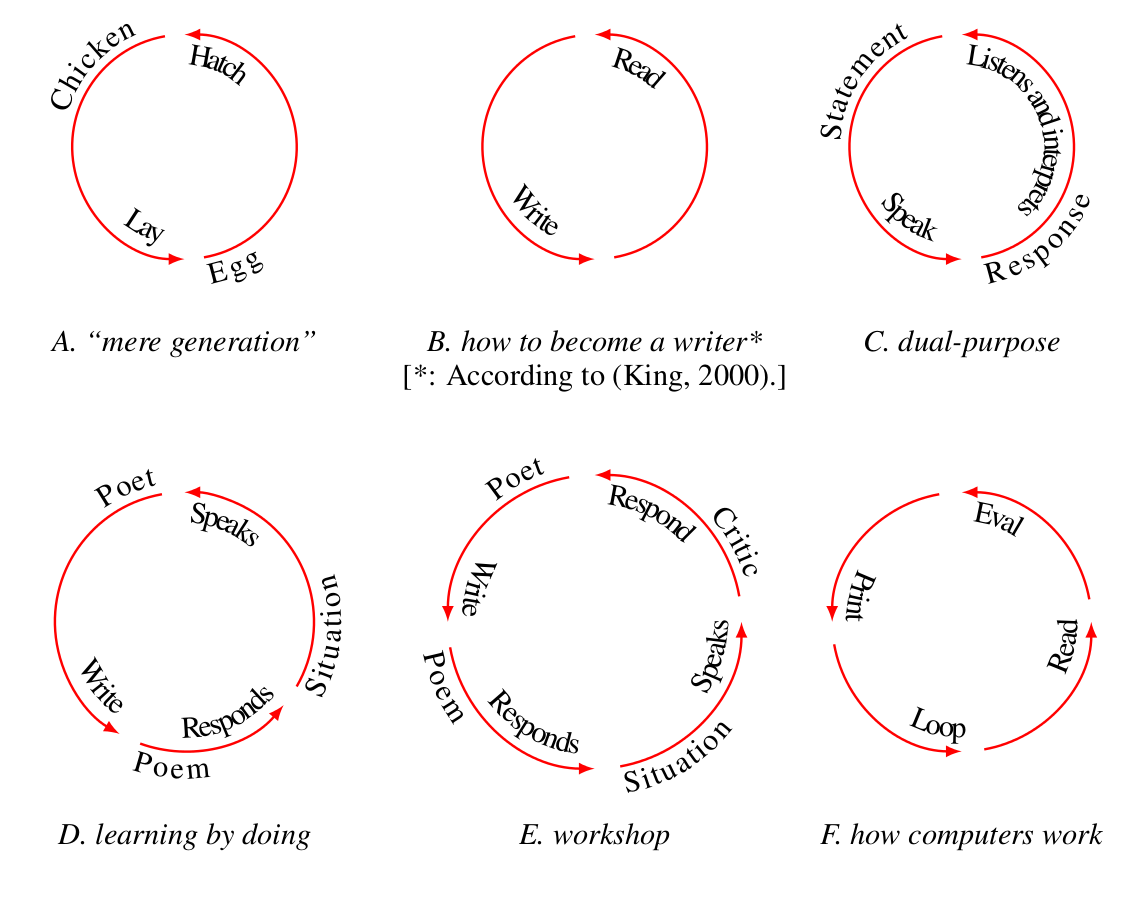
\includegraphics{figures/cycles_shortcut}
}

\caption{(A) gives a simple recipe for the growth and
development of a writer;
(B) \emph{response} always has dimensions that goes beyond the
utterance that is overheard;
(C) adds a \emph{reader} who shares the context with the writer and responds.%, and who responds to this context particularly as it is expressed through the poem
\label{fig:cycles}}
\end{figure}


% Figure \ref{fig:cycles}(A) shows the standard chicken-and-egg problem,
% designed to provoke questions about \emph{evolution};
%%
% 1(B) shows an analogous picture that gives a simple recipe for the growth and
% development of a writer;
%%
% 1(C) is a formally similar diagram that squares up to the metalinguistic features of the situation, showing
% that a \emph{response} (which may be verbal, visceral, physical or
% something else) always has dimensions that goes beyond the utterance that is overheard;
%%
% 1(D) examines in further detail what happens when someone \emph{writes} 
% -- namely, writing as a response to some perceived disturbance, newly identified problem, etc., and writing as it responds to the disturbance does itself become an agent of change;
% Note: we've elided the word "situation" as a totalising concept
%%
% 1(E) adds a \emph{reader} who shares the context with the writer, and who responds to this context particularly as it is expressed through the poem;
% Note: we could call this character a "reader" instead, since "criticism" is pre-judges what they are going to do
% There is another way to read this as related to "crisis" and the different things that can be embedded in
% the poem.
%%
% 1(F) shows that this scenario is not as unfamiliar to computer programmers as it might
% otherwise sound -- consider that the ``Eval'' phase in a
% Read-Eval-Print loop can be interrupted with a debugger to fine-tune
% program operation.

\subsection{``What are the proposed `lab rats'?''}

\footnotetext{According to \citep{king2000writing}.}

% We take as our study of interest the domain of computational poetry. Figure \ref{fig:cycles} illustrates different representations of cyclical processes within creativity, from the simplistic ``mere generation'' through to complex interplays between creator and critic/reader. 

The generative side of the cycles in Figure \ref{fig:cycles} has been studied more than the reflective side.
Our ``lab rats'' are, accordingly, not poems per se, but rather,
\emph{instances of reading and responding to poetry}.  Naturally, such responses could be more or less
``canned'' (as with Michael Cook's humorously nonspecific
AppreciationBot\footnote{\url{https://twitter.com/appreciationbot}}), so the question becomes: what constitutes an
interesting and useful response, and how will these be
developed?  The idea of responses is useful at various levels.
We focus here on staging an encounter between writer and reader.

\subsection{Writer's Workshops}

Quoting \cite[pp. 2--3]{gabriel2002writer}:

\begin{quote}
The original idea behind the writers' workshop was to do a \emph{close
  reading} of a work%, to use the term F. R. Leavis coined for the
%practice of 
... looking at the words on the page rather than the
intentions of the author or the historical and aesthetic context of
the work.  Under this philosophy, the workshop doesn't care much what
the author feels about what he or she wrote, only what's on the page.
%This corresponds to the philosophy of the New Critics, which held that
%the work was its own ``being,'' with its own internal consistency and
%coherence, which could be studied apart from the author.  Moreover,
%this approach is nearly identical to that of the Russian formalists,
%who thought that the proper approach to literature was to study how
%literary texts actually worked, their structures and devices.
\end{quote}

Framing and any other contextualisation of the work \emph{as it is intended to be presented} is permitted, and receives critical attention.
% we described a template for a pattern
% language for interactions in a computational poetry workshop, closely
We define a \emph{Workshop} closely following
Gabriel's outline, to be an activity consisting of these steps:
%itemize?
{\tt presentation}, {\tt listening}, {\tt feedback}, {\tt questions}, and 
 {\tt reflections}.  The first and most important feature of {\tt feedback} is
 for the listener to say what they heard; in other words, what, for them, is in the work.  In some
 settings this is augmented with {\tt suggestions}.  After any
 {\tt questions} from the author, the commentators may make {\tt replies} to offer clarification. 
In related recent work, we have shown how the Workshop framework 
can help foster serendipitous discovery and invention
\cite{serendipity-arxiv,feedback-arxiv}.

%%%%%%%%%%%%%%%%%%%%%%%%%%%%%%%%%%%%%%%%%%%%%%%%%%%%%%%%%%%%%%%%%%%%%%%%%%

\subsection{Content as creative process}
% check title 
\label{sec:philosophy_and_methods}

% \emph{How can a created artefact tell us about its making, and how could this contribute to computational creativity?}

Giving agency to the poem rather than the poet's intentions, the poem illuminates its own creative process.  
This informs our approach to Workshop interactions,
which are focusing on the poem observing its own construction.  We're interested
in context not in the literary or historical sense but in the micro-history of the poem's creative evolution.
% Expand?
% Q
% \emph{Why do we need a model that might enable us to observe the
% creative process in the artistic outcome or practice (e.g.~poems)?}
% A
The originary and therefore unpredetermined nature of
the creative process means that the outcome represents a
more accurate and objective evidence of the process than
the poet's attempt to explain the process. 
% According to Kant,
% the creation of a work of art is rooted in the artist's subjective experience,
% and ``rule and precept are incapable of serving as the requisite subjective standard'' for what makes art \emph{fine} art
% (``Critique of Aesthetic Judgement'', \textsection 57).
Moreover, to the extent that a creator knows what is expressed through the creative process, even he or she learns this only in the course of doing the work.
Observers are only able to consider after the fact how a creator may have selected and rejected various possibilities.   The \emph{content} of the poem is no more and no less than how the poem was made.

\begin{quote}
``In a poem, objective material becomes the content and the matter of the emotion and not
just its evocative occasion.'' \sourceatright{\cite[p. 69]{dewey2005art}}
\end{quote}

P. G. Whitehouse writing on Dewey's \emph{Art as Experience} suggests that Dewey joins
Collingwood in separating aesthetic emotion from any notion of
inspiration that could be considered to be something like raw materials.  
An emotion is
\emph{aesthetic} when it ``adheres to an object formed by an expressive act''
\cite[pp. 149--156]{whitehouse1978meaning}.  However, ``the art
object does not have emotion for its significant content''; rather, the 
emotion
% \begin{quote}
``belongs to the self that is concerned in the movement of events toward an issue that is desired or disliked'' 
%\sourceatright{
\cite[p. 14]{dewey2005art}.%}
%\end{quote}


% ``The painter does not paint; he watches himself paint'' \cite[p. 7]{collingwood1958principles}.
% \subsection{Drivers of the creative process}
% Collingwood uses the term ``oppression'' to describe something that happens to the artist.  Dewey describes this phenomenon as
% ``disturbance'' and Anderson and Hausman see it as a ``colouring'' \cite{anderson1992role}.
%
% The artist becomes conscious of the movement of events and starts to explore his/her own response.
% This is at first an ``intuited feeling'' \cite{kemp2003croce},
% which in the course of expression gives rise to a new feeling of ``alleviation'' or ``easement.''

\subsection{Aspects of the creative process}

Doug Anderson and Carl Hausman take Collingwood's study further and map the
creative process roughly as follows \cite[pp. 299-305]{anderson1992role}:

\begin{quote}
Disturbance $\rightarrow$ aesthetic emotion $\rightarrow$ response $\rightarrow$ artist's decision on components of expression $\rightarrow$ feeling of easement plus a simultaneous emerging of a unique imaginative expression $\rightarrow$ alleviation $\rightarrow$ realising and converting prior psychical emotion $\rightarrow$ unique aesthetic experience including new conscious emotion 
\end{quote}

The poem is a \emph{work of progress} before it is a \emph{work in progress}.
%
The purpose of a poetry workshop that attends to the content of the poem as process is to illuminate what the poet is exploring through his/her creative process and through the poem. The process
of reading a poem is also a process of \emph{poiesis} -- and in the Workshop, the reader joins the writer in the process of creation.  Asking questions like those listed in in Table \ref{tab:questions_for_human_readers} 
tells us what the constituent parts of the poem are doing.

\subsection{Relevance for CC research}

From a CC standpoint, asking what the work tells us about the creative process gives an objective and critical focus on ``creative evolution'' \cite{bergson1983creative} and provides an antidote to the seductions of mere generation.  A poetry workshop gives participants the opportunity to read the drafts and final versions of poems by other Workshop participants, a shared culture of critique that can be applied to previously existing poems, and a structured way to gather feedback on one's own work in progress.  These analyses, unbiased by the explanations of the (software) creator, will allow participants to explore and extend the conceptual space around poetry, or in practical terms, the toolbox the agents can access. ``Extending'' expresses both a refinement of the tools used and the introduction of entirely new tools. Moreover, reverse-engineering of the creative process from artefacts will help to teach agents participating in the workshop at which stage of \textit{their} creative process these new tools or extensions could potentially be used.  Dialogue in the workshop involves ``respecting the voices of each of the participants'' \cite{seikkula2014open}, be they agents, poems, or individual words -- and suggests that we look at the ``art of boundary crossing'' that is to be found \emph{inside} poems.  %Bringing poetry together with dialogue suggests an emphasis on making and using boundary-crossing objects and processes.

\begin{table}[t!]
{\small
\def\arraystretch{1.2}
\begin{tabular}{p{1.8in}p{1.1in}}
\textbf{Question} & \textbf{Examples} \\[.1cm]
What are the register(s) of the poem? & cliched, instructive, imperative\\
Who is addressed? & reader, poet, friend, rival, confidante \\
What position(s) are present in the poem? & pleading, remonstrating, ephemeral\\
What is the poem doing with the reader? & accuse, bewilder, alienate\\
Who are the characters in the poem? & ``the falconer'', ``you'', narrator, ``two men'' \\
What is the role of image(s) in the poem? & ``the sea'', ``a bicycle''; multiple meanings\\
What functions, mechanics, and paradigms are present for the reader to engage with? & communication, subverted cliche\\
What problems, discomforts, or dis-easements are invoked in the poem? & horror, self-loathing, rejection, desire \\
How do these evolve? & E.g. an image may start to take over from a register \\
What is the world of the poem, and how does the poem distinguish between this and its perception of this? & ``Surely'', ``must''; sacred vs mundane; perspectival vs surreal; tale vs telling \\
What are the overlaps, transitions, implicit dialogues? & ``twinned'' lines/ideas, juxtaposed parts of the poem\\
What role does the chronology of reading play, versus references to chronology and chronological positions within the poem? & flagged development, evolution, movement, stasis\\
How are lexical categories used? & solid nouns, tortuous adjectives, indistinct adverbs \\
Are there discernible allusive effects? & illustrating the literary apprenticeship of the author (or reader)\\
Where is the poet presented with respect to the poem? & Confidence, determination, exploration\\
% How does Keats' idea of negative capability feature in the composition -- ``that is when man is capable of being in uncertainties''? & we must also worry about overconfidence and over-determined lines\\
% don't worry about the boyscouts building a fire behind the tree
\end{tabular}
}

\caption{Questions that we ask when reading a poem\label{tab:questions_for_human_readers}}
\end{table}
% \subsection{Connections to Bergsonism}

% Although it is beyond the scope of the current work to trace these connections, we will remark that this view is connected with the
% Bergson's perspectives on creative evolution, and to the genre of philosophy that takes up these themes:
% running to Mead who offers a generalised view of the social,
% to Bakhtin who develops the notion of dialogue in a metalinguistic frame,
% and to Deleuze who develops an ontology based on the idea of difference \cite{bergson1983creative,
%  mead1932philosophy, bakhtin1984problems, deleuze1994difference}.
% These perspectives are relevant to the interest we take here in
% emergence, polyvocality, and learning by specifying and engaging with novel problems.

%%% Local Variables: 
%%% mode: latex
%%% TeX-master: "poetryICCC"
%%% End: 
